\chapter{Egy frekvenciaváltó tervezése}

\paragraph{}

Tesla 1888-ban bemutatott három fázisú indukciós motorjával, nyilvánvalóvá vált, hogy az ilyen típusú gépek megbízhatóbbak és gazdaságosabbak tudnak lenni, mint az egyenáramú motorok. Jelentős hátrányuk azonban, hogy a vezérlésükhöz háromfázisú feszültséget kell előállítani, mely akkoriban csak egy szintén háromfázisú generátor segítségével volt megoldható. Manapság a háromfázisú teljesítmény a villamos hálózatnak köszönhetően rendelkezésre áll, azonban még így is vet fel prooblémákat ezen motorok üzemeltetése.

A frekvenciaváltó egy olyan eszköz mely váltakozó áramú bemenetből váltakozó áramú kimenetet állít elő, mint ahogy a neve is mutatja, más frekvenciával vagy akár feszültséggel, mint a bemenet. Erre azért van szükség, mert a meghajtani kívánt folyamatnak nagyon valószínű, hogy más igényei vannak, mint amit a hálózat önmagában képes biztosítani. Értem ez alatt azt, hogy közvetlen összeköttetés esetén a motorunk $50\ Hz-el$, vagy ennek egész számú hányadosával tudna forogni, illetve ennek a paraméter a befolyásolása fizikailag csak a motor módosításával lehetséges. Természetesen mint az ipar és az élet minden szegmensében itt is célunk a feladat minél hatékonyabb végrehajtása. A világon a teljes villamosenergia felhasználás mint egy $25\ \%-$-át adják a villamos hajtások és ez a szám folyamatosan nő (pl. az elektromos közlekedés térnyerésével). Az igény tehát nyilvánvaló ezeknek az eszközöknek a folyamatos fejlesztésére.

\begin{figure}[!h]
	\centering
	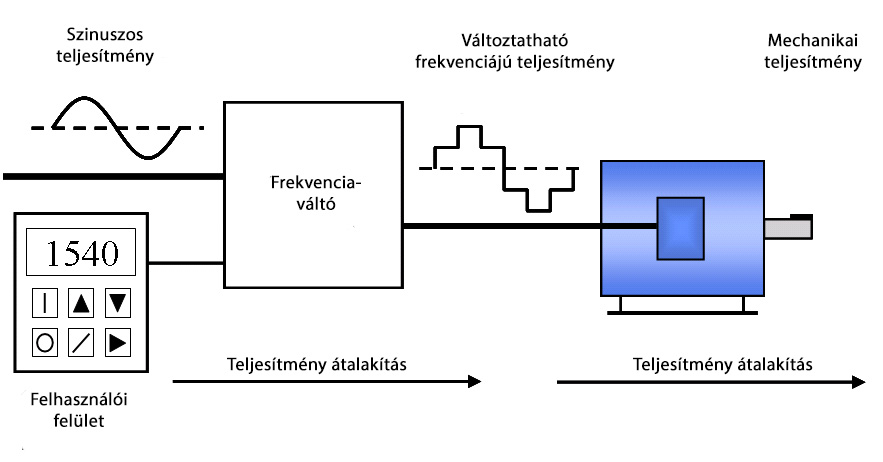
\includegraphics[width = 0.8\textwidth]{figures/VFD_System.jpg}
	\caption{A frekvenciaváltó szerepe} 
	\label{fig:vfd_system}
\end{figure}

Az eszköz feladatát jól összefoglalja \aref{fig:vfd_system} ábra. A hálózatból érkező teljesítményt, a felhasználó által megadott paraméterekkel átalakítjuk, majd a terhelő gépet meghajtuk vele. A modern hajtások ennél jóval szofisztikáltabb működésre is képesek, gondoljunk itt akár távfelügyeletre, identifikációra, vagy esetleg akár vezeték nélküli hozzáférésre.

\paragraph{}
A korábban az ilyen teljesítmény átalakítási feladatokat elektromechanikus berendezésekkel oldották meg, nevezetesen egy motor és generátor párral, ahol is a megfelelő póluspár arány kiválasztásával a frekvenciát módosítani lehetett. Amennyiben szükséges volt feszültségmódosítás is, megfelelő áttételű transzformátor segítségével valósították meg. Ennek a megoldásnak hátránya a nagy teljesítmény esetén nagy méretű villamos gép, ennek megfelelően a kicsi teljesítménysűrűség. A megbízhatóságot csökkenti a mozgó alaktrészek jelenléte és folyamatos igénybevétele, illetve a nagy forgó tömeg is hordoz magában veszélyeket. Ezt követően megjelentek a vákumcsöves eszközök, azonban az igazi áttörést a teljesítményelektronikai félvezető elemek megjelenése okozta.

Ezek a modern eszközök már tartalmaznak mozgó alakrészt (feltéve persze, hogy a reléket és kontaktorokat nem számmítjuk). A félvezető technológia fejlődésével egyre nagyobb és nagyobb teljesítménysűrűségeket tudunk elérni.

\begin{figure}[!h]
	\centering
	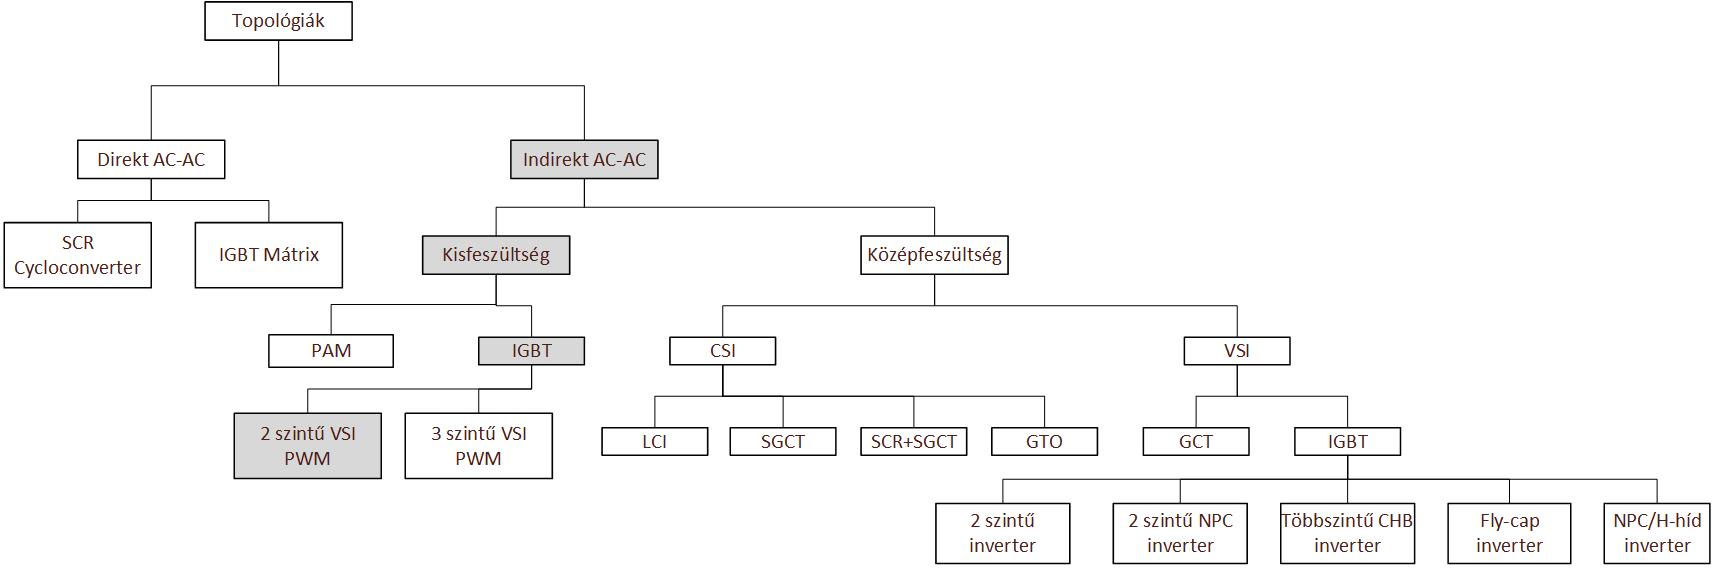
\includegraphics[width = \textwidth]{figures/topologies.jpg}
	\caption{A frekvenciaváltó típusok} 
	\label{fig:topologies}
\end{figure}

\Aref{fig:topologies} ábrán láthatjuk a napjainkban elterjedt inverter típusokat. Az ábrában szürkével kiemeltem a Hyundai által fejlesztett típust.

\section{Termék specifikáció}

A Hyundai által jelenleg fejlesztett frekvenciaváltó család kis feszültségű, általános célú PWM vezérlet IGBT kapcsolóelemű 2 szintű inverteres frekvenciaváltó, passzív front-end-el, azaz a hálózatra nem tud visszatáplálni. \Aref{fig:family} táblázatban látható a jelenleg fejlesztett termékcsalád.

\begin{table}[]
\centering
\begin{tabular}{|c|c|c|c|l}
\cline{1-4}
\textbf{Név} & \textbf{Teljesítmény (kW)} & \textbf{Áram (A)} & \textbf{Tömeg (kg)} &  \\ \cline{1-4}
\multirow{4}{*}{\textbf{FR1}} & 0,55 & 3,7 & \multirow{4}{*}{6} &  \\ \cline{2-3}
 & 0,75 & 4,8 &  &  \\ \cline{2-3}
 & 1,1 & 6,6 &  &  \\ \cline{2-3}
 & 1,5 & 8 &  &  \\ \cline{1-4}
\multirow{3}{*}{\textbf{FR2}} & 2,2 & 11 & \multirow{3}{*}{10} &  \\ \cline{2-3}
 & 3,7 & 18 &  &  \\ \cline{2-3}
 & 5,5 & 25 &  &  \\ \cline{1-4}
\multirow{2}{*}{\textbf{FR3}} & 7,5 & 31 & \multirow{2}{*}{20} &  \\ \cline{2-3}
 & 11 & 48 &  &  \\ \cline{1-4}
\multirow{3}{*}{\textbf{FR4}} & 15 & 62 & \multirow{3}{*}{37,5} &  \\ \cline{2-3}
 & 18,5 & 75 &  &  \\ \cline{2-3}
 & 22 & 88 &  &  \\ \cline{1-4}
\multirow{3}{*}{\textbf{FR5}} & 30 & 114 & \multirow{3}{*}{66} &  \\ \cline{2-3}
 & 37 & 140 &  &  \\ \cline{2-3}
 & 45 & 170 &  &  \\ \cline{1-4}
\multirow{2}{*}{\textbf{FR6}} & 55 & 211 & \multirow{2}{*}{108} &  \\ \cline{2-3}
 & 75 & 261 &  &  \\ \cline{1-4}
\end{tabular}
\caption{A fejlesztés alatt álló termékpaletta}
\label{fig:family}
\end{table}

Azt, hogy a termék milyen széles területét lefedi az iparnak, jól jellemzi, hogy az ezt leíró dokmentum 52 különböző tételt különböztet meg. A teljesség igénye nélkül a felvevő piac néhány szelete:

\begin{itemize}
	\item{Nagyfeszültségű légkondícionálók}
	\item{Élelmiszeripar}
	\item{Textilipar}
	\item{Szállítószalagok}
	\item{Csomagolás és cimkézés}
	\item{Nyomtatás}
	\item{Gépi megmunkálás}
	\item{Autóipar}
\end{itemize}

A hardveres funkcionalitás nagyjából megegyezeik minden esetben, az igazán nagy különbség az egyes területek között a szoftver funkcionalitásában van. Egy szállítószalag esetében fontos a pontos fordulatszám tartása, vagy a pontos pozíció beállítása, míg más felhsználás esetében a potos nyomatékszabályozás lehet fontos, ilyen lehet pl. a villamos vontatás.

Amennyiben külön nincsen jelölve, a dolgozat a továbbiakban az FR1 kódjelű, legkisebb frekvenciaváltóra hivatkozik a példák esetében.

\section{Az eszköz felépítése}

\paragraph{}
A frekvenciaváltó egyenirányítja a bejövő hálózati feszültséget, egy köztes energiatárolóban, az ún. \emph{DC-link} kondenzátorban tárol némi energiát, hogy a feszültség lengésést alacsonyan tartsa, majd egy kimeneti inverterrel előállítja a szükséges jelalakot. Ezt a vázlatot láthatjuk \aref{fig:vfd_schema} ábrán, kiemelve a hálózatot modellező ellenállást és induktivitást.

\begin{figure}[h]
	\centering
	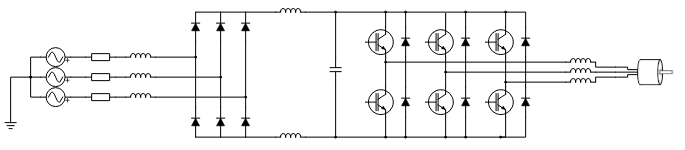
\includegraphics[width = \textwidth]{figures/VFDschematic_choke.png}
	\caption{A frekvenciaváltó egyszerű felépítése} 
	\label{fig:vfd_schema}
\end{figure}

Itt természetesen csak egy vázlatos ábrázolás látató, ezen nem szerepelnek a meghjató elektronikák, a vezérlés, a mérések, és még sok más. Jól látható azonban, hogy a folyamatra egyedül a félhidak vezérlésével tudunk hatni. A Frame 1-ben a kimeneti IGBT-k és diódák egy tokban vannak, egy Semikron SKiiP 24NAB12T4V1 modulban. \cite{sutozoli} \cite{ctan}

\section{A szükséges kompetenciák}

A felépítés alapján elmondható, hogy egy iylen termék összeállítása nagyon bonyolult feladat, sok területet lefed, sok féle kompetenciára van szükség. A teljesítményelektronikai elemek és kapcsolálos megtervezése gyakorlatilag csak az első gondolat. Ezen túl szükséges még a termikus méretezés, a vezérlő elektronikák tervezése, a különböző mérések megvalósítása. Amikor már ezzel is készen vagyunk, akkor a frekvenciaváltó tervezése elektronikai szempontból késznek mondható. Nem sabad megfeledkezni azonban arról, hogy ez egy készülék, melynek a mechnaikus felépítéséről is gondoskodni kell. Itt kerülnek képbe a konstrukcióval foglalkozó gépész kollégák.

\begin{figure}[h]
	\centering
	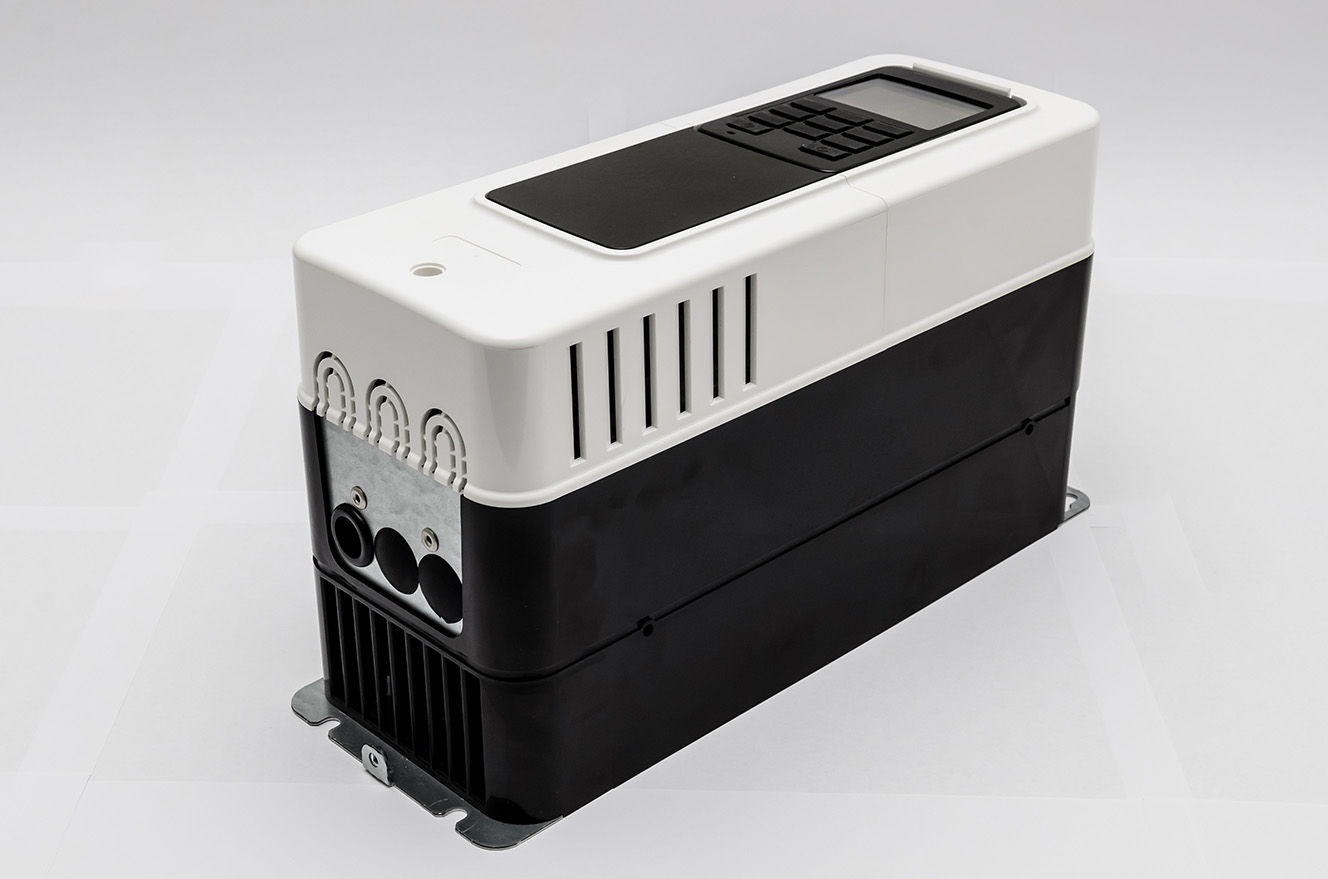
\includegraphics[width = 0.8\textwidth]{figures/n700_proto.jpg}
	\caption{Az elkészült Frame 1 prototípus} 
	\label{fig:n700_proto}
\end{figure}

A feladat már eddig is kellőképpen összett volt, de a termékünk még mindig nem működik. Hiányzik belőlea szoftver, mely önmagában nagyon szerteágazó munka. Először is elő kell állítani a megfelelő szabályzókat, melyek segítsgével elő tudunk állítani színuszos kimenetet, gondoskodni kell a kapcsolóelemek megfelelő modulációjáról. Foglalkozni kell a magasabb szintű funkcionalitás megvalósításával, a különböző kommunikációs vonalak kezelésével, magának a rendszernek a menedzselésével. A HMI\footnote{Human-Machine Interface}-n is meg kell jelenteni információt, biztosíani kell lehetőséget a beavatkozásra. Amennyiben úgy gondolá az olvasó, hogy ez még nem annyira bonyolult, akkor figyelmébe ajánlom a PC-s szoftvert, melyet szintén el kell készíteni, ha egy jól használható terméket kívánunk előálltani. 

\todo[inline]{Félbehagyott gondolat}

\begin{figure}[h]
	\centering
	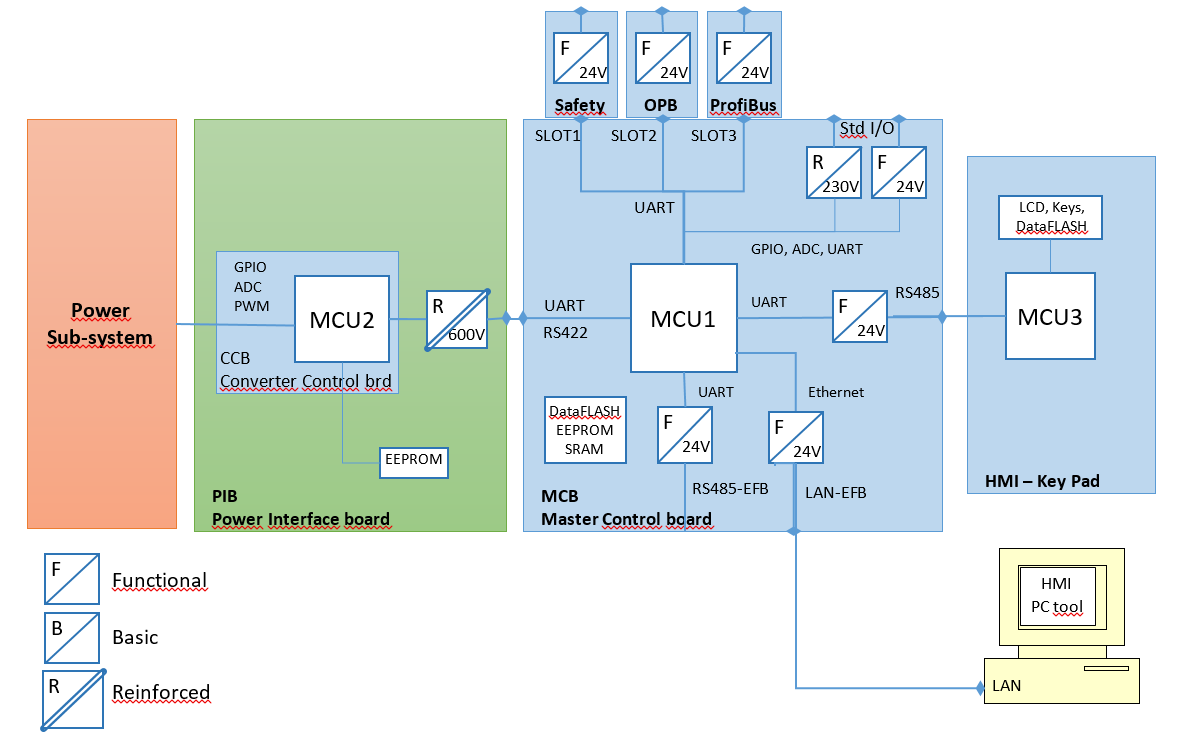
\includegraphics[width = \textwidth]{figures/architect.png}
	\caption{A vezérlő elektronika blokkvázlata} 
	\label{fig:hw_architect}
\end{figure}

\Afigref{hw_architect} ábrán látható a különböző elemek kapcoslata, illetve a kommunikávó közöttük. A CCB feladat a teljesítményátalakítás közvetlen irányítása. Ez a kártya végzi az analóg méréseket, és ezen mérések, illetve a beérkező alapjel alapján előállítja az IGBT-ket vezérlő PWM jeleket. A szoftveres védelmekről is ez a szint gondoskodik. A következő az MCB, mely az egyel magasabb szintű vezérlésért felel. Ez jelenti a kommunikációt más eszközökkel, a különböző terepi buszukon, etherneten, vagy RS-485-ön. Rendelkezik továbbá általános célú digitális és analóg be és kimenetekkel, melyek működése felhasználói igények szerint testre szabható. Ez az eszkösz felelős a számítógépes konfiguráló szoftverrel való kommunikációért, valamint a HMI vezérléséért is. A fejlesztett HIL szimulátor szempontjából ez a három elektronika bír szereppel, ezek közül a HMI csak közvetetten, mivel az MCB-n keresztül kapcsolódik a rendszerhez.

\section{A fejlesztés folyamata}

A teljesítményelektronikai eszközök fejlesztésének a nehézésége abban rejlik, hogy a kisebb teljesítményű modell nem feltéltlenül viselkedik úgy, mint nagyáramú társa. A fenti felíráson az is jól látszik, hogy bizonyos folyamatok párhuzamosíthatóak. A szoftverfejlesztés elkezdődhet a nagyáramú elektornika tervezésésvel együtt, illetve a vezérlő elektronikák is tervezhetően a kezdeti specifiákciók, illetve a a kapcsolódási pontok definiálása után. A fejlődő szoftver teszteléséhez aszonban elengedhetelen, hogy a beágyazott eszköz megkapja a szükséges gerjesztéseket a külvilágtól. Amíg nem áll rendelkezésre a valós eszköz, addig ezt egy szimulátorral vagyunk kénytelenek megvalósítani. Ez a Hardware-in-the-Loop szimulátor. Az eszköz jól jön azonban amikor már a valós frekvenciaváltó is rendelkezésre áll. Az egyes szoftvermódosításokat célszerű kipróbálni ezen az eszközön először, mert egy hiba könnyedén végzetes következményekkel járhat a valós invertren.

\section{Különböző szimulációs eljárások összehasonlítása}

\todo[inline]{Logikai bukfentc, korábban már van HIL, de csak most kezdem kibontani ,hogy mi is az.}

Jól látható tehát, hogy egyértelmű igény mutatkozik valamilyen szimulációs eljárás használatára a fejlesztés minden szakaszában. Természetesen mint minden problémához, ehhez is többféle hozzáállást lehet alkalmazni. Ami mindnekép közös az eljárásokban, hogy a kiváltott hardver-elemek matematikai modelljeit fel kell állítani, azok helyességéről meg kell győződni. A modellezés pontossága és az erőforrás igény között azonban meg kell találni az adott alkalmazásnak és annak szükségleteinek megfelelő kompromisszumot. Elengedhetetlen követelmény azonban, hogy az irányító elektonika szempontjából a modell teljesen transzparens legyen, egyébként nem tudunk reprezentatív következtetést levonni a működés helyességével kapcsolatban. Ez azt jelenti, hogy ugyan azokon az interfészeken keresztül tudjunk a szimulátorral interakcióba lépni, ugyan azokat a válaszokat kapja a szakasztól, mint amit a valóságban is fog kapni, valamint az időzítések is egyezzenek meg az igazi eszközön tapasztaltakkal.

Joggal merül fel a gondolat, hogy asztali számítógépen fontassuk a kifejlesztett modellt, hiszen szokványosan használjuk PC-nket különböző számítások elvégzésére. Nagyon hamar problémába ütközünk. Az első követelmény, hogy rendelkezzen a számítógépünk adatgyűjtő modullal (DAQ - Data Aqusition Module), mely segítségével tudunk mérni és előállítani analóg és digitális jeleket. Ilyen eszközöket lehet kereskedelmi forgalomban kapni, kérdéses azonban a biztosított sávszélesség, a számítógéppel való kommunikáció sebessége, illetve a költsége a vásárolt hardvernek. Ezen felül korlát még az időzítések betartása. Nem is biztos, hogy a számítógépünk valós időben el tudja végezni a szimulációhoz szükséges matekmatikai műveleteket, de ha feltételezzük, hogy igen az egzakt és konzisztens lépésköz egy általános célú asztali számítógépen nem garantálható az operációs rendszer sajátságaiból adódóan. Állnak rendelkezésre valós idejű megoldások, például valós idejű futást támogató Linux kernel, melyet hasonló célra fejlesztettek ki. A számítógép hardveres konfigurációja is korlátot jelent, mert hiába növeljük a processzor teljesítményt, egy ponton túl ($1 - 10 \mu{}s$) a memóriahozzáférések késleltetése miatt nem tudunk kisebb szimulációs lépésközt biztosítani.

A következő lehetőség saját beágyazott hardware fejlesztése, mely emulálja a valós teljesítményelektronikát. Ebben az esteben teljesen testre tudjuk szabni a kapcsolódási pontot, elő tudjuk állítani azokat a jeleket, melyeket vár a vezérlő elektornia, pontosan úgy ahgyo szeretnénk. Előnye a beágyazott processzornak, hogy architektúrájából adódóan garantált futásidőt lehet elérni. A teljesítménye azonban korlátozott az asztali számítógéphez képest, bár, mivel csak egy specifikus feladatot kell végrehajtani, akár még versenyezhet is futásidőben az asztali számítógéppel. Fentiek miatt ez a megoldás leginkább funkcionális tesztek végrehajtására alkalmas, precíz, kvantitatív tesztekre korlátozotan.

A harmadik út - amit részletesebben megvizsgálok dolgozatomban - az FPGA alapú hardware-in-the-loop szimulátor tervezése. Bár a költsége a fejlesztési időt és a hardware költésget tekintve szintén magas lehet, az FPGA architektújából adódóan, nevezetesen létre tudjuk benne hozni az éppen szükséges számításokat elvégző hardvert, rendkívül gyors futásidő érhető el. Ráadásul a PC-vel ellentétben itt az FPGA teljesítményének és órajelének növelésével egyre nagyobb felbontású szimulációt érhetünk elde már a mai technológia is $100 - 10 \ ns$ futásidőre képes.

\begin{figure}[h]
	\centering
	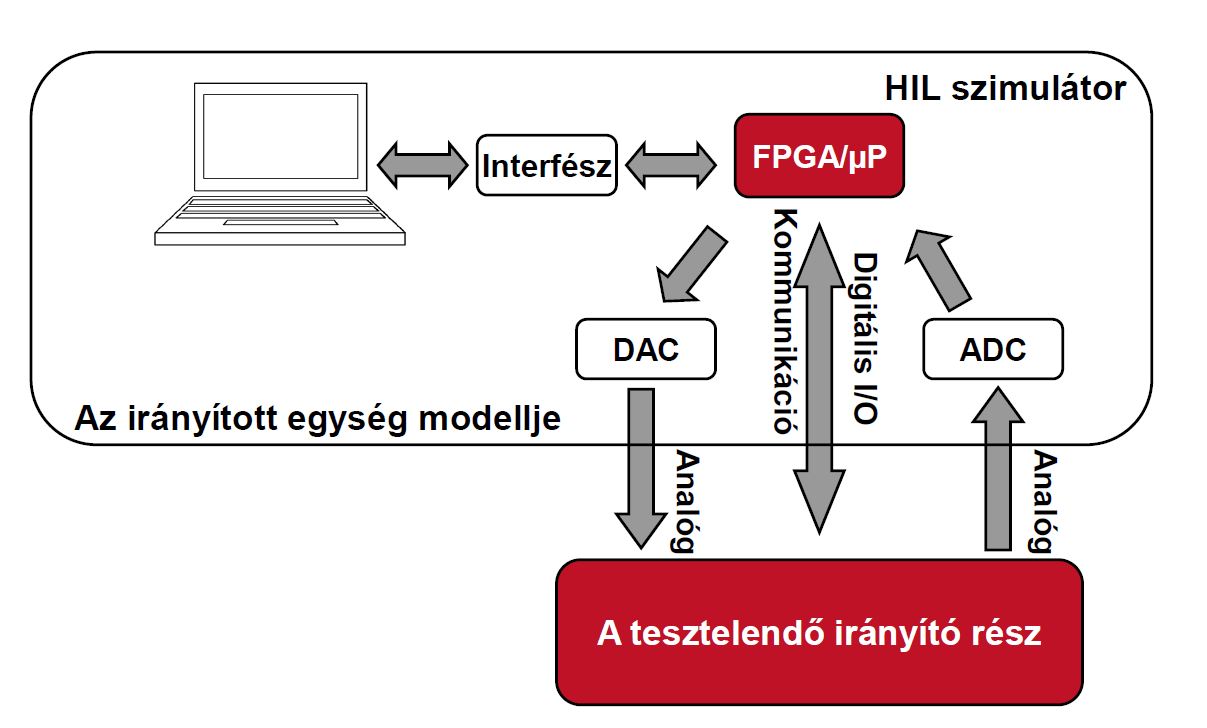
\includegraphics[width = 0.8\textwidth]{figures/hil_idea.png}
	\caption{Az FPGA alapú HIL szimulátor felépítése} 
	\label{fig:hil_idea}
\end{figure}

\todo[inline]{Köki ppt-t behivatkozni}

\section{Szimulációs algoritmusok}

\begin{equation}
\begin{align}
\underline{x}'(t) = \underline{\underline{A}}\cdot \underline{x}(t) + \underline{\underline{B}}\cdot{}\underline{x}(t) \\[0.3em]
\underline{y}(t) = \underline{\underline{C}}\cdot \underline{x}(t) + \underline{\underline{D}}\cdot{}\underline{x}(t)
\end{align} 
\end{equation}

